\documentclass[./Thesis]{subfiles}

\graphicspath{{./Images/}}

\begin{document}


\chapter{Straw Tube Tracking in E989}

In this chapter to explain the work that has been done it is necessary to give a brief introduction to the straw tube tracking fundamentals, the design of the trackers, and the terminology that will be used in later sections. Furthermore, an explanation of the tracking algorithms and how the software used is composed so that there is a further understanding of the motivation and how specifically the goals of the study have been achieved.

\section{Straw Tube Trackers}

The straw tube trackers in gm2 are a fundamental aspect in the measurement Electric Dipole Moment of the muon since these detectors can directly measure the precession tilt of the muon. In addition, the straws are an important part in measuring the beam profile in the experiment and can serve as a double check of the calorimeters. These measurement can be done purely by using the calorimeters in the experiment, however the spatial resolution of the straw trackers will greatly reduce the uncertainty in the measurement.


\subsection{Basic Design of the Straw Tube Trackers}

	A straw tube tracker consist of a series of what is essentially called drift chambers. In general a drift chamber consists  of  an  enclosure  containing  an  anode  and  cathode separated by a region containing a gas. Ref. \cite{aepps} The straws in the detectors consist of mylar tubes which are then with a argon ethane gas and has an anode wire consisting of gold plated tungsten going through the middle of the straws. A diagram of the straw tube and its dimensions is found in Fig.\ref{fig:StrawTube}. For further information of the properties of the straws are given in Fig. \ref{fig:StrawProperties}.
	
\begin{figure}
	\centerline{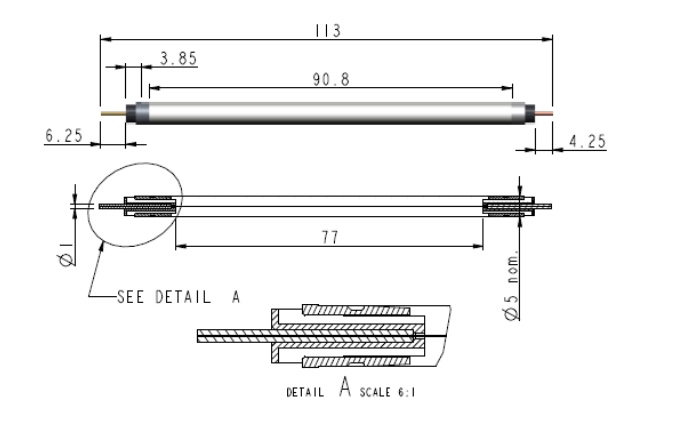
\includegraphics[height=95mm]{StrawTube.jpeg}}
	\caption[ Schematic of Straw Tube]{ A Schematic showing the dimensions of a straw tube Ref. \cite{aepps}
	}
	\label{fig:StrawTube}
\end{figure}

\begin{figure}
	\centerline{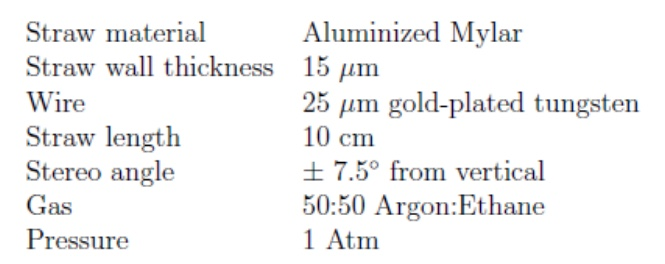
\includegraphics[height=50mm]{StrawProperties.jpeg}}
	\caption[ Table of Straw Properties]{ A table show the properties of a straw Ref. \cite{aepps}
	}
	\label{fig:StrawProperties}
\end{figure}
	
	
	 As a particle passes through the straw the particle interacts ionizes the gas causing the ions to go to the cathode of the straw creating a detectable current. The ions are able to recover electrons from the cathode and the system and returns to a neutral  state. This current can then be measured by the electronics designed for the experiment and can be given to the computer code which will extrapolate the decay position of the particle being detected in the experiment. For further improvement on spatial resolution, the amount of time for the ions to reach the cathode is dependent on where radially in the wire that the particle passes through, this is called the drift time. This drift time can then be extrapolated and added into the track fitting which an explanation of this will be in a later section.  
	 
	 One straw tracker consists of 128 of these straws which are 5 mm in diameter. These 128 straws are then divided up into 4 of what is called layers which are oriented $7.5^\circ$ off the vertical axis with 2 layers being in one direction off the vertical axis and the others layers are in the other direction. This $7.5^\circ$ tilt of the straws allow for the tracking to take this into account an measure the vertical position that the particle hits the detector. This capability is especially important for the EDM measurement. 
	 
	 The Next component of the straw tracker includes what is called the manifold and the flobber.  The straws are then connected to the manifolds which these allow gas to pass through them from one direction and out the other direction. In addition to this the manifold contains the cooling system and the first set of readout electronics. Attached to this manifold are two flanges referred to as the snouts which contain the electronic connections, the cooling system, and allows the gas to flow. Connected to these snouts there are what is called the flobber. The flobber is what houses the majority of the tracker electronics. A diagram of the tracker as a whole is found in Fig. \ref{fig:StrawDetector}.
	
\begin{figure}
	\centerline{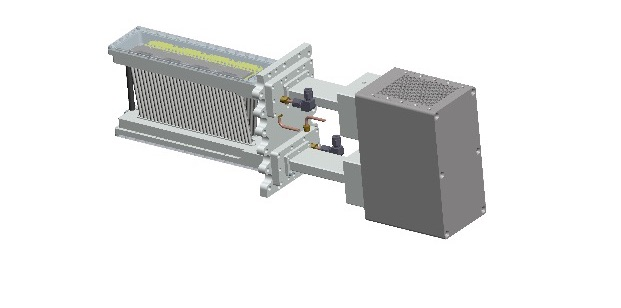
\includegraphics[height=95mm]{StrawDetector.jpg}}
	\caption[ A Straw Detector]{ An example of a straw detector Ref. \cite{TDR}
	}
	\label{fig:StrawDetector}
\end{figure} 

\subsection{Hardware of the Straw Trackers}

	Now that the basic design, reasoning,  and the terminology of the straw trackers themselves is established it is necessary for the systematics discussion to give a basic introduction of the hardware that the tracking system consists of and the terminology of the hardware. In the tracker the straws are connected directly to the ASDQ's which is there to digitize the signal coming from the straw. Fig. \ref{fig:ASDQ} shows an image of one of these ASDQ boards. Every ASDQ board consists of  sixteen straws so therefore there are 8 ASDQ boards serving each tracker.   Flexi-cables are attached directly to the top of the ASDQ boards and route the signal through the snouts to the flobber. A top view of the tracker showing the electronics can be found in Fig. \ref{fig:TopViewTracker} Inside the flobber the signal from the ASDQ boards is then passed to TDC  motherboards. Each motherboard consists of 2 TDC's which connects to one ASDQ. The TDC boards buffer the signal before giving it to the logic boards. Each logic board takes the signal from two TDC's which means that there are four logic boards in a tracker. The logic boards serve as a further buffer for the data,  control the clock,  label the data,  and incorporate data from the low voltage systems. The signal from the logic boards is then passed onto the external electronics located in the flobber. 
	
\begin{figure}
	\centerline{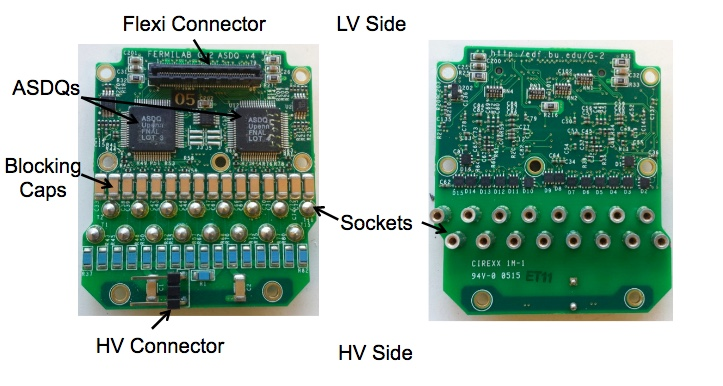
\includegraphics[height=95mm]{ASDQ.jpeg}}
	\caption[Straw Tracker ASDQ]{ An example of a ASDQ board in the trackers Ref. \cite{jmottASDQ}
	}
	\label{fig:ASDQ}
\end{figure} 
	
\begin{figure}
	\centerline{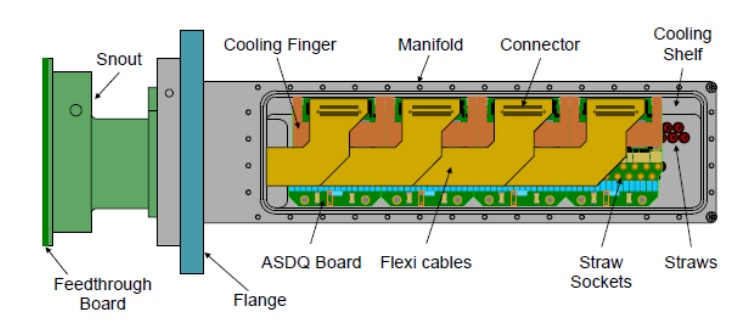
\includegraphics[height=95mm]{TopViewTracker.jpeg}}
	\caption[Top View of Tracker Electronics]{ Cross Section Top View Showing Tracker Electronics  Ref. \cite{jGrange}
	}
	\label{fig:TopViewTracker}
\end{figure} 

	
	The  signal  from  the  logic  boards  is  passed  to  an  FC7  board  housed  in  an  electronics rack and it serves to process the signals coming from the eight trackers at one station. Furthermore, the FC7 board controls the logic board clocks, converts the signal to a readable format for the next electronic board, and passes parts of the signal to a computer which can quickly identify data corruption. The FC7s communicate their data to AMC13 boards which control the clock of the FC7s and communicate the data to the data acquisition system.  A single AMC13 can control all of the tracking stations.
	
\section{Straw Tube Tracking Algorithms}

 	An important part in evaluating the systematics of the straw tube tracking is to understand what the tracking algorithm consists of and how the track fitting process works. In addition, in this section will be an explanation of the data products, what the components of the data products used physically mean, and how those data products are then derived from the tracker data. 
		 
\subsection{Introduction to the Straw Tube Track Finding}

	%%give an introduction to track finding algorithms 


	For each process that the tracking algorithm follows it uses what is called an Art module. Art is an event processing framework used in particle physics. Art is cpp framework that allows different components of code to be used interchangeably, as long as the appropriate data products are being used. In addition, Art allows different constants or processes to be changed throughout the program through one file when running the program rather than changing and compiling different constants throughout the code. This is the main framework for the whole gm2 project and all the other code talked about further is written in this framework.

	The straw tube tracking algorithm consists of the most steps done in processing the data. Although, more complicated and robust than what will be presented the basic idea of the tracking finding is as follows. Coming from the electronics, AMC13, the signal is given to the computer. The computer then gives us a zipped file which consists of what are called rawDigits. These raw digits contain all the information that will be used further in the code and consist of, the TDC time, trigger number, a unique hit ID, TDC ID, FC7 ID, AMC13 ID, ASDQ ID, Logic Board ID, and Channel ID . How the channel ID's are split up can be found in Fig. \ref{fig:channelID}. Each channel corresponds to the same ASDQ and the same Logic board. Every station has the same AMC13 ID. There are 2 TDC's per channel which one TDC would correspond to one layer in a channel. Furthermore, this data product contains what is called the width. The width that is given is the time difference between the rising edge in the wire when current is above a threshold and the falling edge where the current falls below the threshold. 
	
\begin{figure}
	\centerline{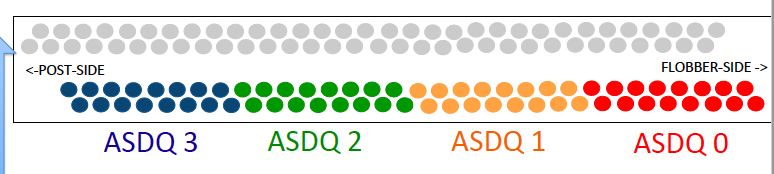
\includegraphics[height=40mm]{ADCSplitUp.png}}
	\caption[Top View of Tracker Electronics]{ Illustration that shows how the channel ID's are split up for each wire  Ref. \cite{jPrice}
	}
	\label{fig:channelID}
\end{figure} 


	
	From this raw data there is a module the makes a more user friendly data product called StrawDigits. From the raw digits, and a geometry file found somewhere else in the code converts the id's to the specific 3d coordinate where the wire is positioned. In addition, from these ID's there is what is called a wireID, which gives an easier format to label wires gives the particular wire that was hit and tells you what station, tracker, layer, view, and wire position of the hit. The convention for number these value goes as follows, there are two stations 12 and 18, there are 8 trackers per station which the lowest number is labeled closest to the ring, there are 2 layers (0,1) looking at Fig. \ref{fig:channelID} the first layer is 0 and the second layer is 1, the third layer is 0 and the 4th layer is 1. There are 2 views in a tracker (0,1) which this corresponds to u or v layer respectively. The wires are labeled from 0-31 with the lowest number being on the left side of the tracker as the particle sees. Lastly this module, also calibrates the TDC times and gives this as the time that hit the tracker. Although, not implemented this was put into place so further reduce down systematics if one of the TDC's get out of time. Lastly, in the strawDigits there consists several other parameters created in this module although they are just filled in as empty to be used later in the code consists of the drift time,  error on the drift time, reconstructed distance of closes approach, and the distance of closest approach error. I will explain these additional parameter later when these parameters are filled with data in the code. 
	
	From the Straw Digits the next module in the algorithm splits these straw hits into 100 ns time intervals into what are called time islands so that the hits are a little bit more manageable. Typically these time island consist between 1 and 4 tracks with very few tracks having 4 tracks but this is given as a maximum value. In addition, this module also extracts what is called the t0, which is the time at which the track hits the first straw in the detector. The t0 has multiple different calculation methods however, it has been found that the best working method for calculation is the average time method where you take the average between the minimum time and the maximum time found in the time island. This value is then adjusted to extrapolate back to where the tracks hits the first layer, telling you at what time the track hits the detector. The time islands data product consists of a unique island ID, the mean time,  minimum time,  maximum time, t0, t0 algorithm ID, t0 success, and the station where the time island occurs. In addition to this, there is a parameter called the upstream digit which stores the wire id of the wire used in the t0 calculation.
	
	Next the time islands are then passed onto the clustering module which groups the digits in the time islands by digits that are neighbor each other. In addition to this from the UV angles and the geometry of the detectors the horizontal position of the track is measured. An example of a cluster pictorially is shown in Fig. \ref{fig:cluster} .  This data product that is passed on has the following parameters to use: mean time, t0 (initial time of cluster), t0 error, the coordinate position of the cluster, horizontal position, horizontal position error, the station number, module, view, and tells if the clusters either overlap with another cluster or if they have shared digits between the cluster. This information is useful for the next module in the process.
	
\begin{figure}
	\centerline{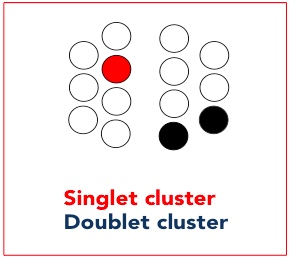
\includegraphics[height=95mm]{Clusters.jpeg}}
	\caption[Cluster Example]{ Examples of Clusters.  Ref. \cite{trackerWiki}
	}
	\label{fig:cluster}
\end{figure} 
	
	
	
	
	The clusters of digits are then processed by the next module which forms what are called seeds. Seeds are derived from clusters which give possible combinations of digits in a particular layer that would belong to a track, ie a track is composed of a multitude of seeds. Fig. \ref{fig:doubleseed} Is a good example of how a cluster could form 2 seeds. The information that is given then from this module consists of: The type of seed (how many seeds belong to that cluster), time , 3d coordinate of the seed, the line slope of the digits on the seed, the line intercept of digits on the seed, if it has shared clusters, station, and whether the first digit is in the front view or the back view.

\begin{figure}
	\centerline{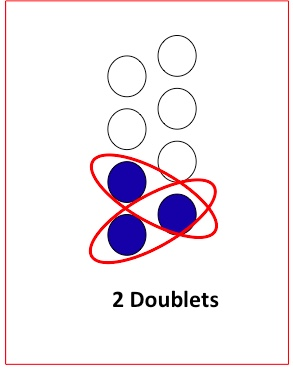
\includegraphics[height=95mm]{doubleseed.jpeg}}
	\caption[Double Seed]{ An example of how you would get two neighboring seeds from one cluster.  Ref. \cite{trackerWiki}
	}
	\label{fig:doubleseed}
\end{figure} 
	
	Probably the most complicated part of the code consists of the next module where this forms what are called track candidates. Track candidates is a single particle track that is derived from the seeds previously established. This is a fairly robust program that can pick out multiple tracks in a time island and forms every possible combination of the seeds a picks out which combinations make physical sense. Shown in Fig. %\ref{fig:trackcandidate} would explain how this algorithm forms different track candidates.
	
\begin{figure}
	\centerline{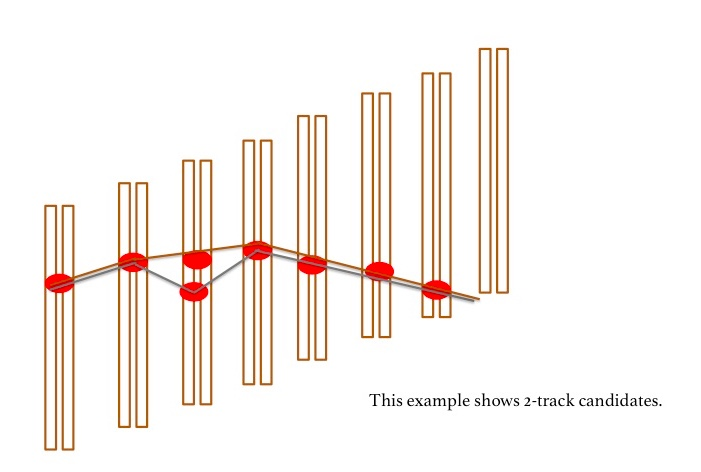
\includegraphics[height=95mm]{trackcandidate.jpeg}}
	\caption[Track Candidate]{ An example of how a track candidates would be formed.  Ref. \cite{trackerWiki}
	}
	\label{fig:trackcandidate}
\end{figure} 
	
	
	Now that the track candidates are selected it is necessary to derive the track t0, drift time, and to reconstruct the distance of closest approach. Similarly, to finding the t0 in the time island the t0 is calculated by finding the average time from the first digit and the last digit in the track candidate and then extrapolating to the time that the first digit in time hits the track. The t0 is an important part to determining the drift time of the hit and therefore the distance of closest approach. The drift time of the straw hit is determined as the difference between the hit time of the straw (which is the average time between rising and falling edge of the current) and the t0. Please refer to Fig. \ref{fig:drifttime}. An example drift time distribution that is normally seen is found in Fig. \ref{fig:drifttimedist} From this drift time now can be determined the distance of closest approach. The distance of closest approach is determined from a physical model that was determined by J. Mott. From an experimental method he looked at a 2d histogram of drift time vs. the distance of closest approach (from the track fitting algorithm not explained yet) as shown in Fig. \ref{fig:driftdca}. In Ref. \ref{jMottdca} he was able to generate this histogram by splitting it up in several regions dependent on the dca. He fitted these function with a gaussian convoluted with an exponential and was able to generate the mean value of the drift time vs. the distance of closest approach. This model then directly converts a drift time to a distance of closest approach with some error.
	
	
\begin{figure}
	\centerline{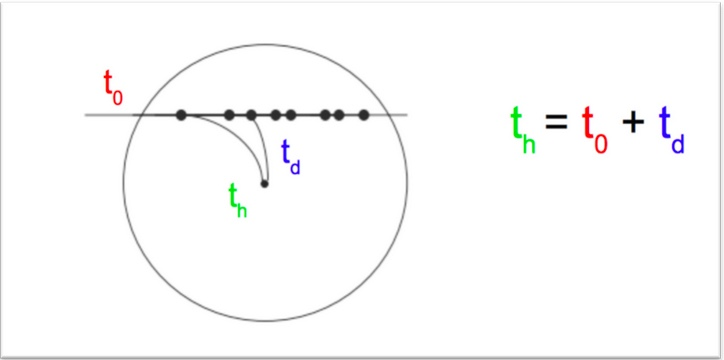
\includegraphics[height=70mm]{drifttime.jpeg}}
	\caption[Drift Time Determination]{ This shows how the drift time distribution by the given t0 and Hit Time  Ref. \cite{trackerWiki}
	}
	\label{fig:drifttime}
\end{figure} 
	
	
\begin{figure}
	\centerline{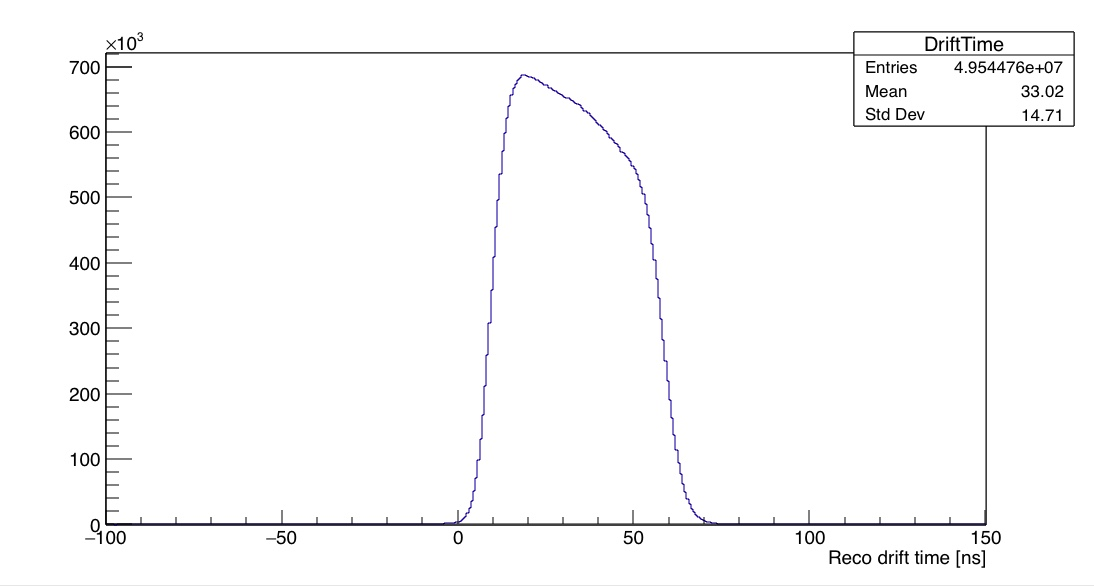
\includegraphics[height=70mm]{drifttimedist.jpeg}}
	\caption[Drift Time Distibution]{ This show what a typical drift time distribution looks like	}
	\label{fig:drifttimedist}
\end{figure} 

\begin{figure}
	\centerline{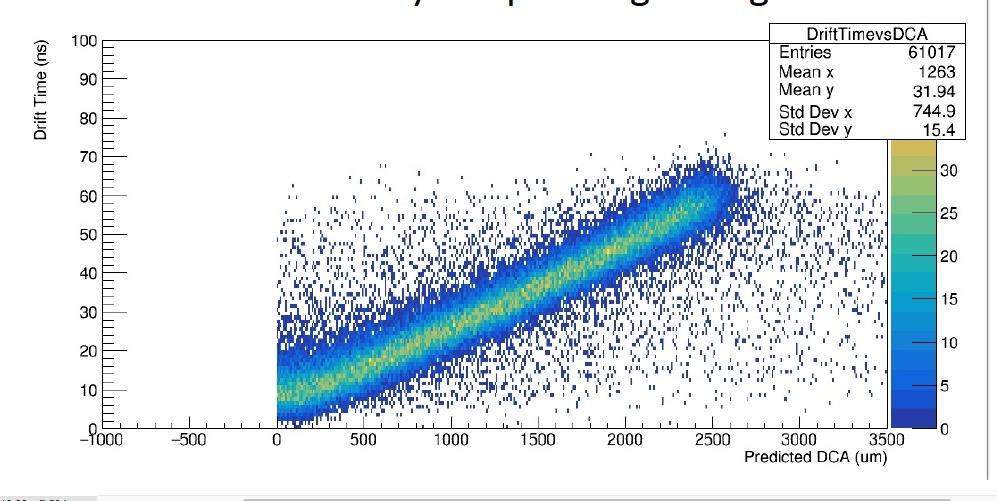
\includegraphics[height=70mm]{driftdca.jpeg}}
	\caption[Drift Time Distibution vs. The distance of closest approach]{ Example histogram of how the distance of closest approach is modeled	}
	\label{fig:driftdca}
\end{figure} 



	In this section was explained the basic tracking process without the track fitting involved. Here in the code all the information necessary has been derived to fit the track and to extrapolate the track to the decay position in the storage ring.

\subsection{Track Fitting and Reconstruction}

	The track fitting and the track reconstruction is a complicated process that I will explain very briefly just to give an idea of what is going on in the tracking. The fitting algorithm used is a standard $\chi^2$ fitting algorithm where there is a starting $\vec{p}$ and then the $\chi^2$ value is minimized to the data. In order to do the fit it is necessary to determine whether the track goes to the left or right of the wire. This is handled by first doing a simple linear fitter between seeds that are doublets. For each doublet the algorithm goes between every different combination of left and right sides of the wire. Then the angle between the lines between neighboring seeds are minimized to one another and those selections of left or right side of the wire is chosen. Now there is a five parameter $\chi^2$ fit described by the variables ($\frac{1}{p},\lambda,\phi,y_\perp,z\_\perp$) here the coordinate system is given by Fig.\ref{fig:geanecoord} . The variable are then transformed using a Jacobian to ($\frac{1}{p},\frac{pu}{px},\frac{pv}{px},u,v$). Then they can be converted from uv coordinates to xy coordinates using another Jacobian. \cite{nickKin}
	
\begin{figure}
	\centerline{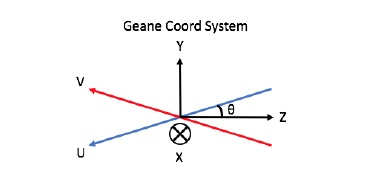
\includegraphics[height=70mm]{GeaneCoord.jpeg}}
	\caption[Geane Coordinate System]{ The Geane Coordinate system used in tracking, z is in direction of the trackers, x is parallel to the tracking planes, z is horizontal Fig.	\cite{nickKin}}
	\label{fig:geanecoord}
\end{figure} 
	
	The track extrapolation algorithm us a Runge-Kutta Nystron algorithm. The algorithm begins with a state vector $\textbf{S}_i$, positions and momentum of the fitted track. These parameters are propagated along a step $\textbf{d}_o$ by evaluating the equation of motion at four immediate stages. The magnetic field information is queried back at each one of these stages. The angles of the track at each stage are weighted to obtain the final state vector at the end of the step. Please Refer to Fig. \ref{fig:extrapstep} for a pictorial representation. After each step the geometry of the ring is queried and flags each track that hits a material in the ring. Also at each step the radial momentum component is evaluated and the extrapolation stops when the radial momentum is zero or when the extrapolated track is parallel with the storage ring. Refer to Fig. \ref{fig:parring} for a cartoon representation. 
	
\begin{figure}
	\centerline{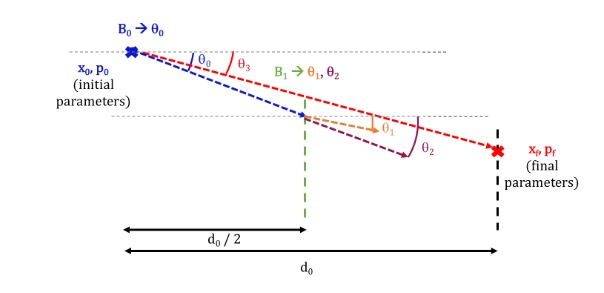
\includegraphics[height=70mm]{ExtrapStep.jpeg}}
	\caption[An Extrapolation Step]{ A pictorial explanation of an extrapolation step	\cite{Sask}}
	\label{fig:extrapstep}
\end{figure} 


\begin{figure}
	\centerline{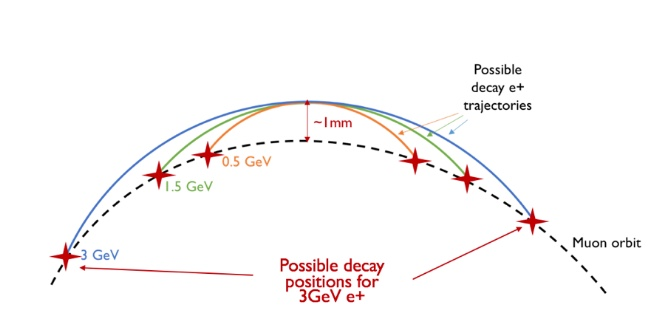
\includegraphics[height=70mm]{ParRing.jpeg}}
	\caption[Radial Momentum zero]{ A pictorial representation of when the radial momentum is zero in gm2 and its possible decay trajectories for different energies \cite{Sask}}
	\label{fig:parring}
\end{figure} 


	
	
\section{Uncertainties in the Straw Tube Detectors}

After the tracking methods have been established it was necessary to understand exactly where the errors are coming from and how much they contribute to the final measurements, since it needs to be established how important certain corrections are to the tracking algorithms or track selection. 

\subsection{Explanation of Uncertainties}

Uncertainties are an important aspect of the gm2 experiment. Significant care has to be taken to ensure that we do not have more than the budgeted errors established in previous sections in any section of the experiment or the experiment will not succeed. Therefore, since the development of the trackers and the tracking algorithms the tracking team has spent a significant amount of time trying to address and characterize different systematical error that may happen in the experiment. This section gives a brief explanation of the errors that are associated with specifically the tracking analysis mainly done by collaborators.

As shown before the main ability of the trackers is to have good spatial resolution as compared to the calorimeters. Therefore, in studying the systematics the main extrapolated quantities of interest is the extrapolated y position (horizontal position) and the radial position (decay point in the ring). All of the important quantities for the experiment that are on a tight error budget are derived from these quantities. Furthermore, for brevity I am only going to cover the final errors contributed to the pitch correction and the electric field correction which use the y and r position respectively. 

	For the pitch correction refer to Table \ref{Tab:PitchErrors}. The single largest error is from the acceptance effects of the trackers which consists of 16 ppb which is larger than all the other systematics being discussed. Looking at the largest error found in Table \ref{Tab:PitchErrors} which is the straw stereo angle this will be deviation of the straws from the idealistic $7.5^\circ$. On a similar scale of this error is the ability to find the Left and Right side of the wire in the track fitting. The next largest error consists Lost muon contamination which are muons hitting the detectors that never decayed into a positron. Internal alignment is the deviation of the individual straw trackers from the idealistic geometry. Close to this is our ability to determine the t0 of the track which was explained previously. 

	 The following errors contribute all on the same level.  Then the hit resolution which will be explain in a later section. The external alignment which is the deviation of the tracker station as a whole from the ideal geometry. The track finding errors are from when we pick the wrong track candidate or a wrong digit. Material effects are from ignoring the fact that the positron is passing through a mylar straw. Lastly, the smallest contribution is the contribution from electronic cross talk which will be discussed in a later section.The other errors we know are there however they have not been currently determined. This consists of variances in the magnetic fringe field near the trackers since this is a derived quantity not a measured quantity. The R to T error is the error being introduced from our distance of closest approach and drift time model variations. \cite{jMottpitch}
	
		In conclusion currently for the pitch correction the total systematic uncertainty $19.3+?$. For the 60 hour data set the tracker it is found that the measured pitch correction is given by $C_p=164.7\pm0.1(stat)\pm21.1+?(syst)$. Although a bit large for the total error budget of 30 ppb for both the E-feild and pitch corrections this is only the first run in the experiment and in the future a lot of these systematics will get much smaller. There is no need to discuss the radial parameter it given in a little different format actual error vs. ppm but you still can get the general idea of how much different aspect contribute. Here it looks like the internal alignment is the greatest contributor to the errors of the electric field contribution. Refer to Fig.\ref{Tab:RadialErrors}
	
		

\begin{table}%[Systematic Error Contribution of the Pitch Correction]
\begin{center}
\caption{Systematic Error Contribution of the Pitch Correction}
\label{Tab:PitchErrors}
\begin{tabular}{ c c }
\hline
Systematical Error		&   Error (ppb)\\
Stereo Angle			&    6.9 \\
L/R					&    6.9 \\
Lost Muon Contamination &	2.9 \\
Internal Alignment		& 	1.5 \\
t$0$					&	0.6\\
Hit Resolution			&	0.3\\
External Alignment		&	0.3 \\
Track Finding			&	0.3 \\
Material Effects			&	0.3 \\
R to T				& 	? \\
Magnetic Fringe Field	&	? \\
Cross-Talk			&	$<$0.005 \\
\hline
\end{tabular}
\end{center}
\end{table}

\begin{table}%[Systematic Error Contribution to the Radial Distribution]
\begin{center}
\caption{Systematic Error Contribution to Radial Disribution}
\label{Tab:RadialErrors}
\begin{tabular}{ c c }
\hline
Systematical Error		&   Error (mm)\\
Stereo Angle			&    ? \\
L/R					&    0.2\\
Lost Muon Contamination &	0.055 \\
Internal Alignment		&	0.162\\
t$0$					&	0.035 \\
Hit Resolution			&	0.03\\
External Alignment		&	0.01\\
Track Finding			&	0.03 \\
Material Effects			&	0.02\\
R to T				& 	0.026 \\
Magnetic Fringe Field	&	? \\
Cross-Talk			&	$<$0.005 \\
\hline
\end{tabular}
\end{center}
\end{table}

		
		
		%%Need to make the table 
	
\end{document}